\documentclass[11pt,letterpaper,spanish]{article}

\usepackage{caption}
\usepackage{float}

\usepackage{iftex}
\ifPDFTeX
  % --- Setup for pdfLaTeX ---
  \usepackage[utf8]{inputenc}
  \usepackage[T1]{fontenc}
\else
  % --- Setup for XeLaTeX & LuaLaTeX ---
  \usepackage{fontspec}
  \setmainfont{Latin Modern Roman}
\fi


\usepackage[spanish]{babel}

\usepackage{url}
\usepackage{hyperref}
\usepackage{geometry}
\usepackage{svg}
\usepackage{fancyhdr}
\usepackage{xcolor}
\usepackage{multicol}
\usepackage{enumitem}

%% Paquetes caseros
\usepackage{customcode}

% ==========================================
% MARCADO DE PROCEDENCIA DE LAS JUSTIFICACIONES
% (permite distinguir lo tomado de Explicación.pdf
%  de las propuestas de mejora para poder depurarlas)
% ==========================================
\definecolor{propcolor}{RGB}{0,90,160}

\tcbuselibrary{breakable}

\newcommand{\marcaOriginal}{}
\newcommand{\marcaPropuesta}{\textnormal{\small\textcolor{propcolor}{(propuesta)}}}

\newtcolorbox{cajapropuesta}{
	colback=propcolor!4,
	colframe=propcolor,
	boxrule=0.5pt,
	arc=2pt,
	left=5pt, right=5pt, top=5pt, bottom=5pt,
	breakable
}



% Required by biblatex-apa for context-sensitive quotes
\usepackage{csquotes}

% Load biblatex with official APA 7th edition style
\usepackage[style=apa, backend=biber]{biblatex}
\addbibresource{referencias.bib}


\geometry{margin=2cm, top=2.5cm, bottom=2.5cm}

\definecolor{headergray}{gray}{0.3}
\definecolor{rulecolor}{gray}{0.6}

\pagestyle{fancy}
\fancyhf{}
\renewcommand{\headrulewidth}{0.5pt}
\renewcommand{\footrulewidth}{0.5pt}
\fancyhead[L]{\small\textcolor{headergray}{UNIVERSIDAD NACIONAL AUTÓNOMA DE MÉXICO}}
\fancyhead[R]{\small\textcolor{headergray}{\documentoTitulo}}
\fancyfoot[L]{\small\textcolor{headergray}{FACULTAD DE CIENCIAS, 2027-I}}
\fancyfoot[C]{\small\textcolor{headergray}{\thepage}}
\fancyfoot[R]{\small\textcolor{headergray}{FUNDAMENTOS DE BASES DE DATOS}}

% ==========================================
% CONFIGURACIÓN DE VARIABLES (EDITAR AQUÍ)
% ==========================================
\newcommand{\documentoTitulo}{Tarea 03}
\newcommand{\documentoSubtitulo}{Modelo Relacional}

\newcommand{\profesorNombre}{Gerardo Avilés Rosas}

\newcommand{\ayudanteTeoriaUno}{Oscar Daniel Flores Linares}
\newcommand{\ayudanteTeoriaDos}{Claudia Itzel Gutiérrez Sánchez}

\newcommand{\ayudanteLabUno}{Ricardo Badillo Macías}
\newcommand{\ayudanteLabDos}{Rocío Aylin Huerta González}

\newcommand{\equipoNombre}{Dobles Comillas}

\newcommand{\integranteUno}{Contreras Morales Román Ismael}
\newcommand{\integranteDos}{Cornejo de la mora Iñaki}
\newcommand{\integranteTres}{Hipólito Felipe Christopher Guillermo}
\newcommand{\integranteCuatro}{Ledesma Cuevas Eduardo}

% ==========================================

\begin{document}

\thispagestyle{empty}

\begin{center}
	\vspace*{1cm}

	\begin{tabular}{cc}
		
\includegraphics[width=3cm]{escudos/unam_seal.pdf} & 
\includegraphics[width=3cm]{escudos/fc_seal.pdf}
	\end{tabular}

	\vspace{0.8cm}
	{\LARGE\bfseries UNIVERSIDAD NACIONAL AUTÓNOMA DE MÉXICO}\\[0.3cm]
	{\large FACULTAD DE CIENCIAS, 2027-I}\\[0.3cm]
	{\large\bfseries FUNDAMENTOS DE BASES DE DATOS}

	\vspace{1.2cm}
	{\huge\bfseries \documentoTitulo:}\\[0.3cm]
	{\Large \documentoSubtitulo}

	\vspace{1.5cm}
\end{center}

\begin{multicols}{2}
	\raggedcolumns

	\textbf{PROFESOR:}\\
	\profesorNombre\\[1.2cm]

	\textbf{AYUDANTES DE TEORÍA:}\\
	\ayudanteTeoriaUno\\
	\ayudanteTeoriaDos\\[1.2cm]

	\textbf{AYUDANTES DE LABORATORIO:}\\
	\ayudanteLabUno\\
	\ayudanteLabDos\\[1.2cm]

	\columnbreak

	\textbf{EQUIPO:}\\
	\equipoNombre\\[1.2cm]

	\textbf{INTEGRANTES DEL EQUIPO:}\\
	\integranteUno\\
	\integranteDos\\
	\integranteTres\\
	\integranteCuatro

\end{multicols}

\vspace{1cm}

\section*{Preguntas De Repaso}
\begin{enumerate}[i.]
	\item ¿Qué es una relación y qué características tiene?

	      En el modelo relacional, una relación es una tabla que representa un conjunto de entidades o de asociaciones entre ellas.

	      Matemáticamente, una relación es un subconjunto del producto cartesiano de $n$ dominios \[A_1 \times A_2 \times \dots \times A_n\]
	      donde cada posición corresponde a un atributo cuyo dominio es $A_i$.

	      De esta forma, un elemento de la relación (llamado tupla) se identifica con una entidad (o asociación entre entidades) que tiene asociados ciertos valores para cada atributo.


	      De manera más simple, podemos pensar a una relación simplemente como una tabla bidimensional, donde cada columna representa un atributo y cada renglón representa un elemento de dicha relación.

	      Las características principales son:
	      \begin{itemize}
		      \item Cada fila representa una instancia individual, por lo que no pueden haber filas idénticas repetidas.

		      \item Cada columna representa un atributo.
		      \item Cada celda de la tabla (equivalentemente, cada elemento de algún $A_i$) es indivisible, es decir, no pueden ser listas ni arreglos.
		      \item No existe un orden específico entre las filas de la tabla. Es decir, la relación efectivamente es un conjunto (sin orden).
		      \item El orden de las columnas tampoco es significativo.

	      \end{itemize}


	\item ¿Qué es un esquema de relación?
	      Es la estructura o el diseño de la relación: el nombre de la relación y el conjunto de sus atributos, junto con el dominio de cada uno. Describe qué se almacena, no los datos concretos.



	\item ¿Qué es una llave primaria?, ¿qué es una llave candidata?, ¿qué es una llave mínima?, ¿qué es una super llave?
	      Conviene explicar en el orden inverso.
	      Una superllave es cualquier conjunto de atributos de una relación que permiten identificar de forma única a cada tupla de la relación. Es decir, no pueden existir dos tuplas con exactamente los mismos valores en dichos atributos.
	      A menudo las superllaves contienen información redundante, es decir, no se requieren todos los atributos de la superllave para identificar unívocamente a las tuplas de la relación.

	      Si nos enfocamos en superllaves que no contienen información redundante, llegamos al concepto de llave mínima:
	      es un conjunto de atributos que permiten identificar unívocamente a los elementos de la relación, y tal que quitar cualquier atributo de la llave rompe esta propiedad.

	      Una llave candidata es una llave mínima; se le llama candidata porque cualquiera de ellas puede elegirse como llave primaria.

	      Finalmente, una llave primaria es una llave candidata elegida por el diseñador para identificar a los elementos de la relación. Su valor es el que las llaves foráneas de otras relaciones referencian para vincular tuplas.


	\item ¿Qué restricciones impone una llave primaria y una llave foránea al modelo de datos relacional?

	      Como ya mencionamos, una llave primaria debe ser capaz de identificar de manera única a los elementos de la relación. Además de esto, no se permiten valores nulos en los atributos de una llave primaria.

	      Por otro lado, una llave foránea es un conjunto de atributos de una relación cuyos valores deben coincidir con los de una llave primaria (o candidata) de otra relación (o incluso de la misma), o bien ser nulos.
	      La restricción más importante que impone el uso de una llave foránea es la integridad referencial: salvo los nulos, cada valor de la llave foránea debe existir como llave de alguna tupla de la relación referenciada.


	\item Investiga cuáles son las Reglas de Codd y explica con tus propias palabras cada una de ellas. Indica por qué consideras que son importantes.


	      \begin{enumerate}[start=0, label=\textbf{Regla \arabic*.}]
		      \item \textbf{(Fundacional):} Un sistema manejador de bases de datos relacional debe administrar todos sus datos usando únicamente sus capacidades relacionales, sin depender de mecanismos de bajo nivel.
		      \item \textbf{(Información):} Toda la información debe representarse de una sola manera: como valores dentro de tablas.
		      \item \textbf{(Acceso garantizado):} Todo valor debe poder recuperarse combinando el nombre de la tabla, el valor de la llave primaria de la fila y el nombre de la columna.
		      \item \textbf{(Valores nulos):} Debe poder representarse la información faltante o inaplicable con un valor nulo, distinto de cero o de la cadena vacía y válido para cualquier dominio.
		      \item \textbf{(Catálogo dinámico en línea):} La descripción de la base de datos (sus metadatos) debe almacenarse en tablas y poder consultarse o modificarse con el mismo lenguaje que los datos ordinarios.
		      \item \textbf{(Sublenguaje de datos completo):} Debe existir un lenguaje textual que permita, de forma interactiva y desde programas, definir datos y vistas, manipular datos, expresar restricciones de integridad, gestionar autorizaciones y delimitar transacciones.
		      \item \textbf{(Actualización de vistas):} Toda vista cuya actualización sea teóricamente posible debe poder actualizarla el sistema.
		      \item \textbf{(Operaciones de alto nivel):} El sistema debe operar sobre conjuntos completos de filas a la vez, no obligar a procesarlas una por una.
		      \item \textbf{(Independencia física):} Los programas y consultas no deben verse afectados por cambios en la forma en que los datos se almacenan físicamente.
		      \item \textbf{(Independencia lógica):} Debe poder modificarse la estructura lógica de las tablas sin alterar la manera en que los usuarios acceden a los datos, apoyándose en las vistas.
		      \item \textbf{(Independencia de la integridad):} Las restricciones de integridad deben poder declararse en el propio lenguaje relacional y almacenarse en el catálogo, no programarse en cada aplicación.
		      \item \textbf{(Independencia de la distribución):} El usuario y las aplicaciones no deben poder distinguir si los datos residen en un solo sitio o están fragmentados y distribuidos geográficamente.
		      \item \textbf{(No subversión):} Si el sistema ofrece acceso de bajo nivel, ese acceso no debe permitir violar las restricciones de integridad ni las reglas de seguridad relacionales.
	      \end{enumerate}

	      Estas reglas definen con precisión qué significa que un sistema manejador de bases de datos sea verdaderamente relacional y, por lo tanto, constituyen un estándar y una meta a la que aspirar. Un sistema que las cumple garantiza que el acceso a los datos no dependa de los detalles de implementación física, que la integridad y la consistencia se preserven mediante restricciones declaradas dentro de la propia base de datos, y que exista una interfaz uniforme para consultarla y modificarla. En la práctica, ningún sistema manejador de bases de datos comercial las satisface por completo, por lo que sirven como referencia para evaluarlos.



\end{enumerate}


\section*{Modelo Relacional}
\begin{enumerate}
    \item Concideraciones para Modelo Relacional:
    
    \begin{enumerate}

        \item \textbf{Colección}: Su llave primaria es el atributo \textit{nombre}, con dominio \textit{varchar} con una restricción de integridad de entidad (\textbf{NOT NULL}, \textbf{UNIQUE}). Sus atributos \textit{descripción}, \textit{tipo} y \textit{contacto} operan bajo el dominio \textit{varchar} con restricción \textbf{NOT NULL}.

        \item \textbf{Telefono\_Coleccion}: Se crea a partir de un atributo multivaluado de Colección, entonces su llave es compuesta por la llave de Colección y \textit{teléfono}. El atributo \textit{nombre\_coleccion} (dominio \textit{varchar}) actúa simultáneamente como llave foránea (\textbf{FK}) hacia la relación Colección, aplicando una restricción de integridad referencial. El atributo \textit{telefono} pertenece al dominio \textit{varchar} con restricción de dominio (\textbf{NOT NULL}).

        \item \textbf{Interactuar}: Al ser una relación muchos a muchos se crea esta tabla cuya llave primaria es compuesta por las llaves de las entidades participantes: \textit{nombre\_coleccion} e \textit{idMuseo}. El atributo \textit{nombre\_coleccion} (\textit{varchar}) funciona como llave foránea (\textbf{FK}) hacia la relación Colección, mientras que el atributo \textit{idMuseo} (\textit{int}) funciona como llave foránea (\textbf{FK}) hacia la relación Museo. Ambas imponen restricciones de integridad referencial.

        \item \textbf{Museo}: Su llave primaria es \textit{idMuseo}, perteneciente al dominio de los enteros (\textit{int}) y cuenta con una restricción de integridad de entidad (\textbf{NOT NULL}, \textbf{UNIQUE}). El atributo compuesto Dirección fue descompuesto en sus componentes indivisibles: \textit{calle}, \textit{numero}, \textit{cp} y \textit{estado}. Todos estos atributos, al igual que el atributo descriptivo \textit{nombre}, operan bajo el dominio de cadena de caracteres (\textit{varchar}), bajo restricciones de integridad de dominio (\textbf{NOT NULL}).

        \item \textbf{Teléfono\_Museo}: Se crea a partir del atributo multivaluado \textit{teléfono} de Museo. Su llave es compuesta por la llave \textit{idMuseo} (con dominio \textit{int}) con restricción de integridad referencial; y su llave principal \textit{teléfono} (con dominio \textit{varchar}) con restricción \textbf{NOT NULL}.

        \item \textbf{Obra}: Esta tabla se debe conservar por eficiencia, pues tiene un atributo multivaluado y dos especializaciones. Su llave primaria es \textit{idObra}, perteneciente al dominio de los enteros (\textit{int}) con una restricción estricta de integridad de entidad (\textbf{NOT NULL}, \textbf{UNIQUE}). Sus atributos \textit{titulo}, \textit{descripcion} y \textit{tipo} pertenecen al dominio \textit{varchar}, contando con restricciones de integridad de dominio (\textbf{NOT NULL}). Al tener una cardinalidad de 1:N con participación total en sus asociaciones con Museo, Colección y Artista, la tabla absorbe las llaves de esas 3 entidades. Entonces, integra tres llaves foráneas (\textbf{FK}): \textit{idMuseo} (\textit{int}) derivada de la relación Poseer, \textit{nombre\_coleccion} (\textit{varchar}) derivada de Tener, y \textit{nombre\_artista}, \textit{paterno\_artista}, \textit{materno\_artista} (todos \textit{varchar}) derivados de Crear (las 3 con restricción de integridad referencial).

        \item \textbf{Material\_Obra}: Se creó a partir del atributo multivaluado (\textit{material}) en Obra, por eso tiene una llave compuesta por la llave de Obra y \textit{material}. El atributo \textit{idObra} pertenece al dominio de los enteros (\textit{int}) y actúa simultáneamente como llave foránea (\textbf{FK}) hacia la relación Obra, aplicando una restricción de integridad referencial. El atributo \textit{material} adopta el dominio de cadena de caracteres (\textit{varchar}) con una restricción de integridad de dominio (\textbf{NOT NULL}).

        \item \textbf{Exhibir}: Esta tabla surge de la conversión de una cardinalidad de muchos a muchos (M:N) entre las entidades Obra y Exhibición. Su llave primaria es compuesta por los identificadores de las entidades que conecta: \textit{idObra} e \textit{idExhibicion}. El atributo \textit{idObra} (\textit{int}) y el atributo \textit{idExhibicion} (\textit{int}) fungen simultáneamente como llaves foráneas (\textbf{FK}) hacia sus respectivas relaciones de origen, con restricciones de integridad referencial. Finalmente, se incorporan los atributos de la relación, \textit{fecha\_inicio} y \textit{fecha\_fin}, operando ambos bajo el dominio \textit{date} con restricción de integridad de dominio (\textbf{NOT NULL}).

        \item \textbf{Especialización parcial disjunta}: El modelo conceptual presenta una jerarquía de especialización para la entidad Obra basada en su clasificación física (Pintura, Escultura, Miscelanea). Esta jerarquía se identifica como parcial disjunta. Por eso se crea una tabla para cada una de las tres subentidades. Cada nueva tabla incorpora como llave primaria el atributo \textit{idObra} (\textit{int}). Este identificador actúa simultáneamente como llave foránea (\textbf{FK}) hacia la superentidad Obra, estableciendo una restricción de integridad referencial. La Escultura recibe los atributos \textit{estilo} y \textit{dimensiones} (\textit{varchar}), así como el atributo físico \textit{peso} (\textit{decimal}); Pintura recibe \textit{estilo} y \textit{genero} (\textit{varchar}); y Miscelanea recibe \textit{pais} y \textit{formato} (\textit{varchar}). Todos estos atributos operan con una restricción de integridad de dominio (\textbf{NOT NULL}).

        \item \textbf{Tecnica\_Pintura}: Esta tabla se crea a partir del atributo multivaluado (\textit{técnica}) de Pintura. Su llave primaria es compuesta y está integrada por \textit{idObra} y \textit{tecnica}. El atributo \textit{idObra} (\textit{int}) actúa al mismo tiempo como llave foránea (\textbf{FK}) hacia la relación Pintura, aplicando una restricción de integridad referencial. El atributo \textit{tecnica} adopta el dominio \textit{varchar} con restricción de integridad de dominio (\textbf{NOT NULL}).

        \item \textbf{Especialización total disjunta}: El modelo E-R presenta una segunda jerarquía de especialización para la entidad Obra, clasificada por su estatus de propiedad en las subentidades Permanente y Prestada. A diferencia de la clasificación física, esta jerarquía se identifica como una especialización total disjunta. Las tablas resultantes, Permanente y Prestada, incorporan como llave primaria a \textit{idObra} (\textit{int}), la cual funciona simultáneamente como llave foránea (\textbf{FK}) hacia la superentidad Obra. Esta llave asegura la integridad referencial. La tabla Permanente aloja los atributos \textit{costo} (\textit{decimal}) y \textit{fecha\_adq} (\textit{date}). Por su parte, la tabla Prestada aloja el atributo \textit{prestador} (\textit{varchar}) y los atributos temporales \textit{fecha\_pres} y \textit{fecha\_dev} (ambos de dominio \textit{date}). Todos los atributos atómicos en ambas tablas operan bajo una restricción de integridad de dominio estricta (\textbf{NOT NULL}).

        \item \textbf{Artista}: Su llave principal es \textit{NombreC}, el cual es un atributo compuesto por \textit{Nombre}, \textit{Paterno} y \textit{Materno}, entonces su llave son esos 3 atributos. Todos adoptan el dominio \textit{varchar} con restricción de integridad de entidad (\textbf{NOT NULL}). Los atributos temporales \textit{nacimiento} y \textit{defuncion} se asignan al dominio \textit{date}, mientras que los atributos descriptivos \textit{pais}, \textit{epoca} y \textit{descripcion} operan bajo el dominio de cadena de caracteres (\textit{varchar}). Todos los atributos aplican una restricción de integridad de dominio para evitar valores nulos.

        \item \textbf{Estilo\_Artista}: Se crea a partir del atributo multivaluado \textit{estilo} de Artista. Su llave primaria es compuesta, uniendo el identificador completo de la entidad fuerte dominante (\textit{nombre}, \textit{paterno}, \textit{materno}) con su propio discriminante (\textit{estilo}). Los tres atributos que conforman el nombre fungen simultáneamente como llave foránea (\textbf{FK}) hacia la relación Artista, aplicando integridad referencial. El atributo \textit{estilo} adopta el dominio \textit{varchar} con restricción de integridad de dominio (\textbf{NOT NULL}).

        \item \textbf{Exhibición}: Su llave primaria es \textit{idExhibicion}, la cual se define bajo el dominio de los enteros (\textit{int}) con una restricción estricta de integridad de entidad (\textbf{NOT NULL}, \textbf{UNIQUE}). Su atributo \textit{titulo} pertenece al dominio de cadena de caracteres (\textit{varchar}) y opera con una restricción de integridad de dominio (\textbf{NOT NULL}).

    \end{enumerate}

    \begin{figure}[htbp]
        \centering
        % Ajusta el 0.9 al tamaño que prefieras (ej. 1.0 para ocupar todo el ancho)
        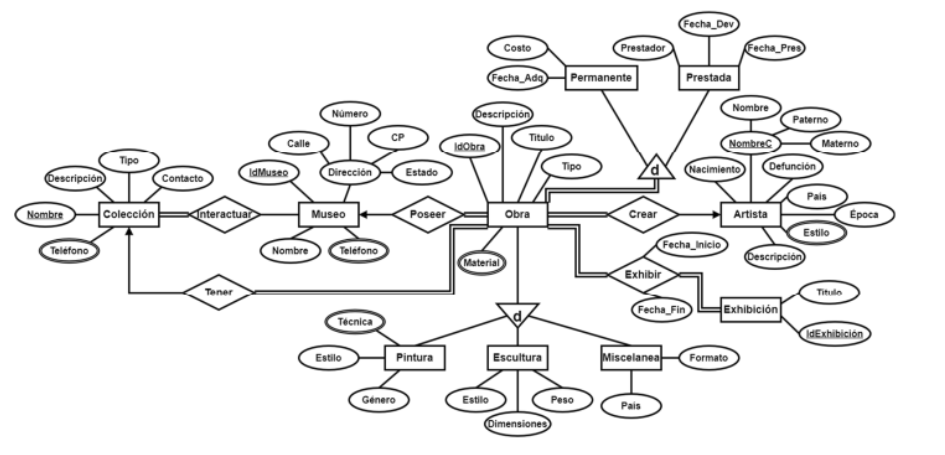
\includegraphics[width=0.9\textwidth]{Figuras/ER_2a.png}
        \caption{Modelo E-R correspondiente al inciso a).}
        \label{Modelo E-R inciso a}
    
    \end{figure}

    \begin{figure}[htbp]
        \centering
        % Ajusta el 0.9 al tamaño que prefieras (ej. 1.0 para ocupar todo el ancho)
        \includegraphics[width=0.9\textwidth]{Diagramas/2_a.drawio.png}
        \caption{Modelo Relacional correspondiente al inciso a).}
        \label{fig:modelo_relacional}
    
    \end{figure}

    \newpage



    \item  Concideraciones para el Modelo E-R
    \begin{enumerate}

  \item \textbf{ELEMENTO\_GEOLÓGICO} (supertipo): \texttt{id\_elemento\_geológico} (llave).
	\item \textbf{RÍO} (subtipo de \textit{ELEMENTO\_GEOLÓGICO}): \texttt{nombre}, \texttt{descripción}, \texttt{longitud\_total}.
	\item \textbf{MONTAÑA} (subtipo de \textit{ELEMENTO\_GEOLÓGICO}): \texttt{nombre}, \texttt{descripción}, \texttt{altura}.
	\item \textbf{MONTAÑA\_VOLCÁNICA} (subtipo de \textit{MONTAÑA}): \texttt{tipo\_volcán}.
	\item \textbf{MONTAÑA\_PLEGAMIENTO} (subtipo de \textit{MONTAÑA}): \texttt{periodo\_geológico}.
	\item \textbf{MUNICIPIO}: \texttt{id\_municipio} (llave), \texttt{nombre}, \texttt{num\_habitantes}.
	\item \textbf{SISTEMA\_MONTAÑOSO}: \texttt{código} (llave), \texttt{nombre}, \texttt{orientación} \{norte, sur, este, oeste\}, \texttt{longitud}, \texttt{altura\_máxima}.
	\item \textbf{SATÉLITE}: \texttt{id\_satélite} (llave), \texttt{nombre}, \texttt{descripción}.
	\item \textbf{ATRAVIESA} (relación N:M entre \textit{RÍO} y \textit{MUNICIPIO}, atributo \texttt{longitud\_tramo}): participación total de \textit{RÍO}, parcial de \textit{MUNICIPIO}.
	\item \textbf{ES\_AFLUENTE\_DE} (relación ternaria recursiva entre \textit{RÍO}, \textit{RÍO} y \textit{MUNICIPIO}): roles \texttt{afluente} (0,1), \texttt{recibe} (0,N) y \texttt{confluencia} (0,N).
	\item \textbf{PERTENECE\_A} (relación N:1 entre \textit{MONTAÑA} y \textit{SISTEMA\_MONTAÑOSO}): participación total de \textit{MONTAÑA}; \textit{SISTEMA\_MONTAÑOSO} es el lado de cardinalidad 1.
	\item \textbf{OCUPA} (relación N:M entre \textit{SISTEMA\_MONTAÑOSO} y \textit{MUNICIPIO}): participación total de \textit{SISTEMA\_MONTAÑOSO}, parcial de \textit{MUNICIPIO}.
	\item \textbf{SE\_ENCUENTRA\_EN} (relación N:M entre \textit{MONTAÑA} y \textit{MUNICIPIO}): participación total de \textit{MONTAÑA}, parcial de \textit{MUNICIPIO}.
	\item \textbf{MONITOREA} (relación 1:N entre \textit{SATÉLITE} y \textit{ELEMENTO\_GEOLÓGICO}, atributo \texttt{fecha\_inicio\_monitoreo}): \textit{SATÉLITE} es el lado de cardinalidad 1; participación parcial de \textit{ELEMENTO\_GEOLÓGICO}.

  
\end{enumerate}

% ==========================================
% Modelo E-R (página en horizontal, tamaño carta)
% ==========================================
\clearpage
% Página tamaño carta en horizontal: se fija el tamaño físico de la página y se
% centra el diagrama, dejando 1 cm de margen por lado.
\pdfpagewidth=11in
\pdfpageheight=8.5in
\setlength{\textwidth}{\dimexpr\pdfpagewidth-2cm\relax}
\setlength{\hsize}{\dimexpr\pdfpagewidth-2cm\relax}
\setlength{\oddsidemargin}{\dimexpr(\pdfpagewidth-\textwidth)/2 - 1in\relax}
\setlength{\evensidemargin}{\oddsidemargin}
\setlength{\textheight}{\dimexpr\pdfpageheight-2cm\relax}
\setlength{\vsize}{\dimexpr\pdfpageheight-2cm\relax}
\setlength{\headheight}{0pt}
\setlength{\headsep}{0pt}
\setlength{\topmargin}{\dimexpr(\pdfpageheight-\textheight)/2 - 1in\relax}
\thispagestyle{empty}
\vspace*{\fill}
\centering
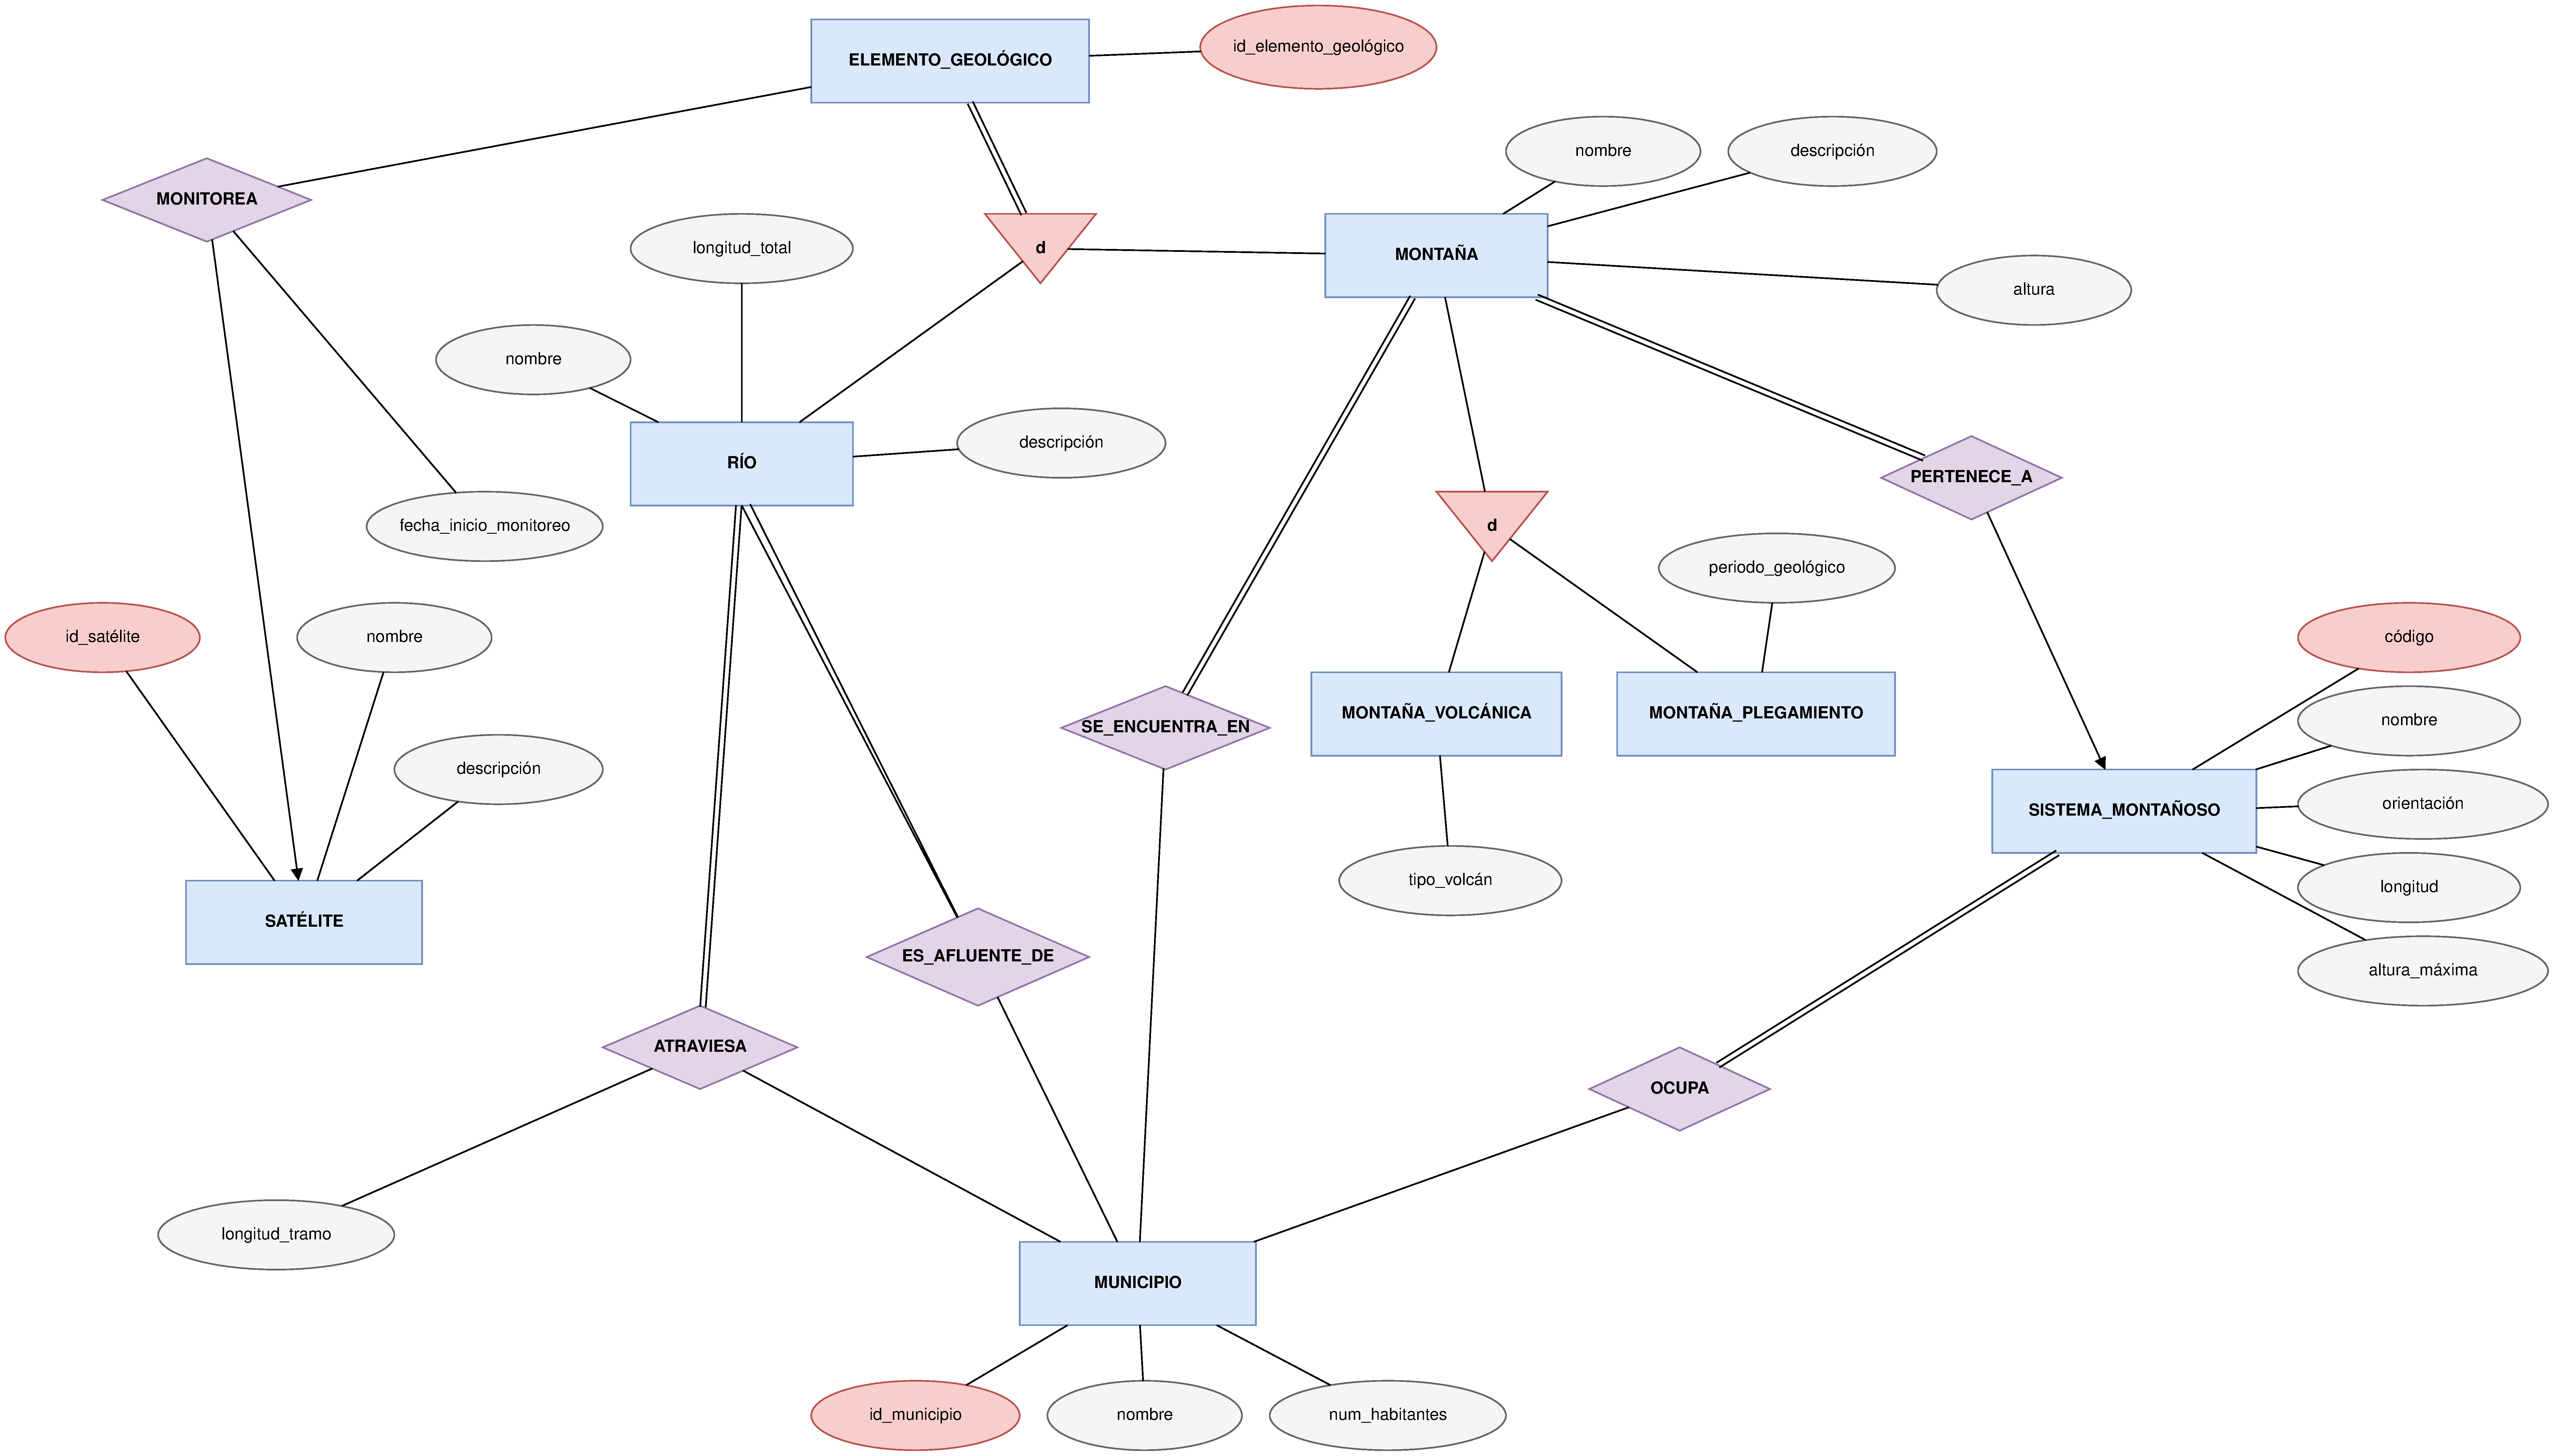
\includegraphics[width=\textwidth, height=0.85\textheight, keepaspectratio]{Figuras/3c.pdf}
\captionof{figure}{Modelo E-R para Sistema de Informacion Geografica.}
\label{fig:er_3c}
\vspace*{\fill}
\clearpage
\restoregeometry
\pdfpagewidth=\paperwidth
\pdfpageheight=\paperheight

\subsection*{Consideraciones para Modelo Relacional}

\begin{enumerate}

\item \textbf{Satélite}: Su llave primaria es \textit{id\_satélite}, perteneciente al dominio de los enteros (\textit{int}) y cuenta con una restricción de integridad de entidad (\textbf{NOT NULL}, \textbf{UNIQUE}). Sus atributos \textit{nombre} y \textit{descripción} operan bajo el dominio de cadena de caracteres (\textit{varchar}) con restricción de integridad de dominio (\textbf{NOT NULL}).

\item \textbf{Municipio}: Su llave primaria es \textit{id\_municipio}, con dominio \textit{int} y restricción de integridad de entidad (\textbf{NOT NULL}, \textbf{UNIQUE}). Los atributos \textit{nombre} (\textit{varchar}) y \textit{num\_habitantes} (\textit{int}) operan con restricción \textbf{NOT NULL}.

\item \textbf{Sistema\_Montañoso}: Su llave primaria es \textit{código}, asumiendo un dominio \textit{varchar} o \textit{int}, con restricción estricta de integridad (\textbf{NOT NULL}, \textbf{UNIQUE}). Sus atributos \textit{nombre} y \textit{orientación} pertenecen al dominio \textit{varchar}, mientras que \textit{longitud} y \textit{altura\_máxima} adoptan el dominio \textit{decimal} (o \textit{int}), todos contando con restricciones de integridad de dominio (\textbf{NOT NULL}).

\item \textbf{Elemento\_Geológico} (Supertipo): Esta tabla funge como el supertipo creado para simplificar los identificadores de \textbf{Río} y \textbf{Montaña}, y para evitar duplicar la relación MONITOREA. Su llave primaria es \textit{id\_elemento\_geológico}, perteneciente al dominio de los enteros (\textit{int}) con restricción (\textbf{NOT NULL}, \textbf{UNIQUE}).
Al tener una cardinalidad 1:N en su asociación MONITOREA con \textbf{Satélite}, la tabla absorbe la llave de dicha entidad. Por lo tanto, integra la llave foránea (FK) \textit{id\_satélite} (\textit{int}) aplicando integridad referencial hacia \textbf{Satélite}. Dado que la participación de \textbf{Elemento\_Geológico} en esta relación es parcial, esta llave foránea admite valores nulos (\textbf{NULL}). Finalmente, el atributo de la relación, \textit{fecha\_inicio\_monitoreo}, es arrastrado hacia esta tabla operando bajo el dominio \textit{date}.

\item \textbf{Especialización total disjunta} (Río y Montaña): El modelo E-R presenta una jerarquía de generalización/especialización total disjunta para la superentidad \textbf{Elemento\_Geológico} en las subentidades \textbf{Río} y \textbf{Montaña}. Se crea una tabla para cada una de las dos subentidades. Ambas incorporan como llave primaria el atributo \textit{id\_elemento\_geológico} (\textit{int}), que actúa simultáneamente como llave foránea (FK) hacia la superentidad \textbf{Elemento\_Geológico} con estricta integridad referencial.
\begin{itemize}
    \item \textbf{Río}: Recibe los atributos propios \textit{nombre}, \textit{descripción} (\textit{varchar}) y \textit{longitud\_total} (\textit{decimal}) con restricción \textbf{NOT NULL}.
    \item \textbf{Montaña}: Recibe los atributos \textit{nombre}, \textit{descripción} (\textit{varchar}) y \textit{altura} (\textit{decimal}). Adicionalmente, al participar en la relación N:1 (PERTENECE\_A) con participación total hacia \textbf{Sistema\_Montañoso}, esta tabla absorbe la llave de dicha entidad. Por tanto, integra la llave foránea (FK) \textit{código} (\textit{varchar}) con restricción de integridad referencial y restricción \textbf{NOT NULL}.
\end{itemize}

\item \textbf{Especialización disjunta} (Montaña\_Volcánica y Montaña\_Plegamiento): Existe una segunda jerarquía de especialización disjunta a partir de \textbf{Montaña}. Las tablas resultantes, \textbf{Montaña\_Volcánica} y \textbf{Montaña\_Plegamiento}, heredan como llave primaria y foránea (FK) simultánea a \textit{id\_elemento\_geológico} (\textit{int}), asegurando la integridad referencial hacia \textbf{Montaña}.
\begin{itemize}
    \item \textbf{Montaña\_Volcánica}: Aloja el atributo \textit{tipo\_volcán} (\textit{varchar}) con restricción \textbf{NOT NULL}.
    \item \textbf{Montaña\_Plegamiento}: Aloja el atributo \textit{periodo\_geológico} (\textit{varchar}) con restricción \textbf{NOT NULL}.
\end{itemize}

\item \textbf{Atraviesa}: Esta tabla surge de la conversión de una cardinalidad de muchos a muchos (N:M) entre \textbf{Río} y \textbf{Municipio}. Su llave primaria es compuesta por los identificadores de las entidades que conecta: \textit{id\_elemento\_geológico} (FK hacia \textbf{Río}) e \textit{id\_municipio} (FK hacia \textbf{Municipio}). Ambas imponen restricciones de integridad referencial. Se incorpora a esta tabla el atributo de la relación \textit{longitud\_tramo}, bajo el dominio \textit{decimal} con restricción \textbf{NOT NULL}.

\item \textbf{Ocupa}: Al ser una relación muchos a muchos (N:M) entre \textbf{Sistema\_Montañoso} y \textbf{Municipio}, se crea esta tabla de intersección. Su llave primaria es compuesta por \textit{código} (FK hacia \textbf{Sistema\_Montañoso}) e \textit{id\_municipio} (FK hacia \textbf{Municipio}), ambas manteniendo integridad referencial estricta.

\item \textbf{Se\_Encuentra\_En}: Al igual que las anteriores, surge de la cardinalidad muchos a muchos (N:M) entre \textbf{Montaña} y \textbf{Municipio}. Su llave primaria es compuesta por \textit{id\_elemento\_geológico} (FK hacia \textbf{Montaña}) e \textit{id\_municipio} (FK hacia \textbf{Municipio}), aplicando restricciones de integridad referencial.

\item \textbf{Es\_Afluente\_De}: Se crea a partir de una relación ternaria recursiva con cardinalidad M:N entre las entidades \textbf{Río} (que participa con dos roles) y \textbf{Municipio}. Su llave primaria es compuesta por los identificadores de los tres roles involucrados: \textit{id\_afluente} (FK hacia \textbf{Río}, dominio \textit{int}), \textit{id\_recibe} (FK hacia \textbf{Río}, dominio \textit{int}) e \textit{id\_municipio} (FK hacia \textbf{Municipio}, dominio \textit{int}). Las tres columnas aplican restricciones estrictas de integridad referencial hacia sus respectivas tablas de origen.

\end{enumerate}

% ==========================================
% Modelo Relacional (página en horizontal, tamaño carta)
% ==========================================
\clearpage
\pdfpagewidth=11in
\pdfpageheight=8.5in
\setlength{\textwidth}{\dimexpr\pdfpagewidth-2cm\relax}
\setlength{\hsize}{\dimexpr\pdfpagewidth-2cm\relax}
\setlength{\oddsidemargin}{\dimexpr(\pdfpagewidth-\textwidth)/2 - 1in\relax}
\setlength{\evensidemargin}{\oddsidemargin}
\setlength{\textheight}{\dimexpr\pdfpageheight-2cm\relax}
\setlength{\vsize}{\dimexpr\pdfpageheight-2cm\relax}
\setlength{\headheight}{0pt}
\setlength{\headsep}{0pt}
\setlength{\topmargin}{\dimexpr(\pdfpageheight-\textheight)/2 - 1in\relax}
\thispagestyle{empty}
\vspace*{\fill}
\centering
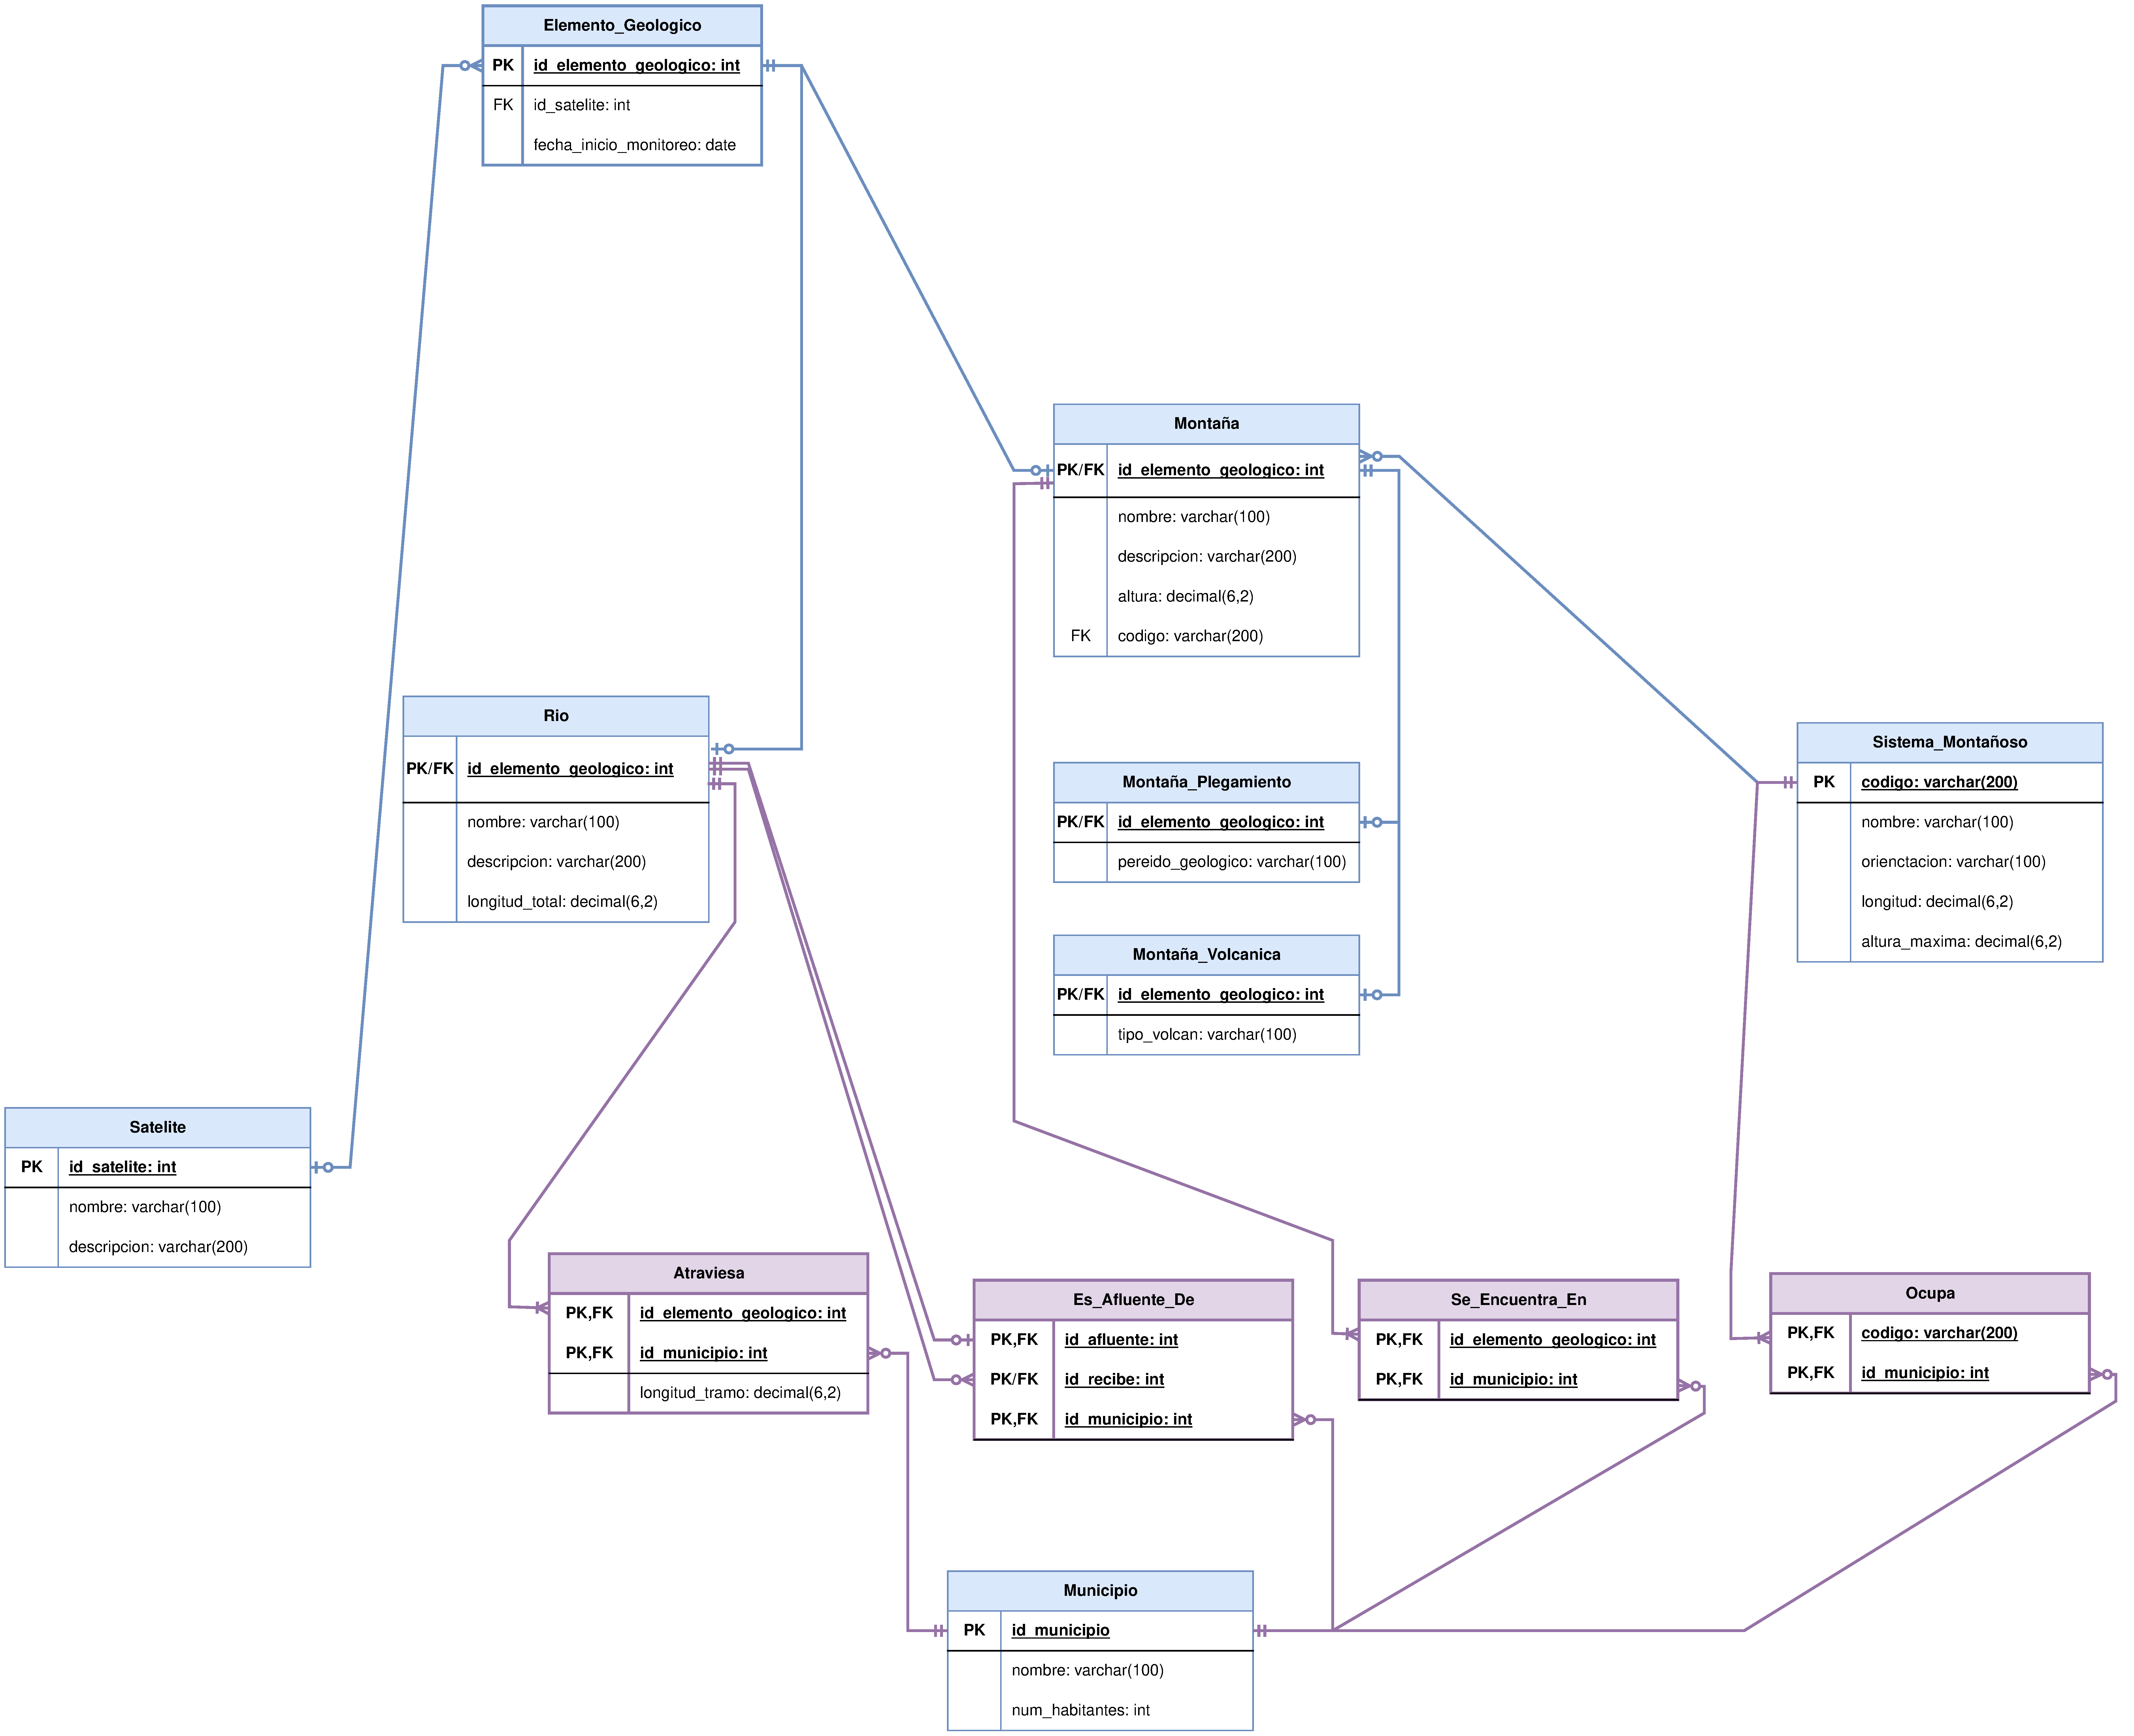
\includegraphics[width=\textwidth, height=0.85\textheight, keepaspectratio]{Figuras/RelacionalT2E3c.pdf}
\captionof{figure}{Modelo Racional para Sistema de Informacion Geografica.}
\label{fig:rel_3c}
\vspace*{\fill}
\clearpage
\restoregeometry
\pdfpagewidth=\paperwidth
\pdfpageheight=\paperheight

\end{enumerate}

\section*{Modelo Relacional e inserción de tuplas}
\begin{enumerate}[a.]
\item \begin{center} \begin{tabular}{|c|c|}
  \hline \\
  Modelo E-R & Modelo Relacional \\
  \hline \\
  M : N & A(a1, a2, a3) B(b, b1) ab(a1, a2, b, ab1) \\
             & A: PK(a1, a2) \\
             & B: PK(b) \\
             & ab: PK(a1, a2, b) FK1(a1, a2) → A(a1, a2) FK3(b) → B(b)  \\
  \hline \\
  1 : N & A(a1, a2, a3) B(b, b1, ab1, a1, a2) \\
             & A: PK(a1, a2) \\
             & B: PK(b) FK1(a1, a2) → A(a1, a2) \\
  \hline \\
  N : 1 & A(a1, a2, a3, ab1, b) B(b, b1) \\
             & A: PK(a1, a2) FK1(b) → B(b) \\
             & B: PK(b) \\
  \hline \\
  1 : 1 & A(a1, a2, a3) B(b, b1) ab(a1, a2, b, ab1) \\
             & A: PK(a1, a2) \\
             & B: PK(b) \\
             & ab: PK(a1, a2, b) FK1(a1, a2) → A(a1, a2) FK3(b) → B(b)  \\
  \hline
\end{tabular}
\end{center}

\item \begin{itemize}
  \item A: (2, 'ww', 'a'); (4, 'xx', 'b'); (6, 'yy', 'c'); (8, 'zz', 'd')
  \item B: (17,  ); (27,  ); (37,  ); (47,  ); (57,  )
  \end{itemize}
  \begin{enumerate}[i.]
  \item Este conjunto de tuplas no se puede insertar debido a que la última tupla repite la PK de la tercera así que viola la restricción de llave primaria. Nos basta con insertar una tupla que relacione dos elementos antes no relacionados (en lugar de la última tupla original) para quedarnos con el conjunto: (8, 'zz', 17, 5); (6, 'yy', 57, 10); (4, 'xx', 27, 15); (2, 'ww', 37, 20); (4, 'xx', 37, 15)

  \item Con este formato ninguna tupla es válida: a1 no existe en A, b no existe en B y ab1 viola la restricción de dominio (cadena en vez de entero). Tomando las cadenas de letras como la tupla correspondiente de A podemos construir fácilmente el conjunto: (8, 'zz', 17, 77); (6, 'yy', 27, 78); (4, 'xx', 37, 79); (2, 'ww', 47, 80); (8, 'zz', 57, 81)

  \item Podemos ver que los pares (2, 'a'), (4, 'b'), (6, 'c') y (8, 'd') no corresponden a ningun (a1, a2) en A por lo que las tuplas no son válidas. Podemos tomar el mismo conjunto de tuplas y sólo reemplazar a3 por a2 para obtener: (2, 'ww', 17, 23); (4, 'xx', 27, 24); (6, 'yy', 37, 25); (8, 'zz', 47, 26); (2, 'ww', 57, 27)

  \item Finalmente tenemos ¡un conjunto válido! Todas las (a1, a2) existen en A al igual que todas las b en B. Finalmente, todas las PKs son distintas.
  \end{enumerate}

\item A falta de detalles sobre el ejercicio, asumimos que A contiene las tuplas del inciso anterior, que B está vacía, que aplican las restricciones de tipo del inciso anterior ($b, ab1, a1$ enteros; $b1, a2$ cadenas) y que tomamos como referencia para las tuplas de B el orden estricto de (b, b1, ab1, a1, a2), es decir, (entero, cadena, entero, entero, cadena).

  \begin{enumerate}[i.]
  \item Este conjunto no se puede insertar. Desde la primera tupla se viola la restricción de dominio, ya que a1 y a2 toman los valores 'zz' y 10, lo mismo ocurre en las demás tuplas. Aun si reordenamos las columnas, los pares (a1, a2) como (57,'zz') o (47,'yy') no existen en A y la última tupla repite la PK b=2. Un conjunto que sí se puede insertar es: (17, 'f', 10, 2, 'ww'); (27, 'g', 20, 4, 'xx'); (37, 'h', 30, 6, 'yy'); (47, 'i', 40, 8, 'zz'); (57, 'j', 50, 2, 'ww')

  \item Este conjunto no se puede insertar. Desde la primera tupla, b1=8 y ab1='zz' violan la restricción de dominio  y a1='f' tampoco es un entero. Con el orden estricto, ninguna tupla es válida. Si se reordenaran las columnas como (b, a1, a2, b1, ab1) el conjunto sí sería válido pero eso contradice el orden asumido. Un conjunto que sí se puede insertar es: (57, 'f', 2, 8, 'zz'); (47, 'g', 4, 6, 'yy'); (37, 'h', 6, 4, 'xx'); (27, 'i', 8, 2, 'ww'); (17, 'j', 6, 6, 'yy')

  \item Este conjunto no se puede insertar. Con el orden estricto, la primera tupla viola el dominio con a1='zz'. Aunque se reordenaran las columnas como (b, b1, a1, a2, ab1), las FK (a1, a2) sí existirían en A pero se repiten las PK b=27 (tuplas 2 y 4) y b=17 (tuplas 1 y 5), lo cual viola la restricción de llave primaria. Un conjunto que sí se puede insertar es: (17, 'f', 1, 8, 'zz'); (27, 'g', 2, 6, 'yy'); (37, 'h', 3, 4, 'xx'); (47, 'i', 4, 2, 'ww'); (57, 'j', 5, 6, 'yy')

  \item Este conjunto sí se puede insertar. Todas las tuplas respetan los dominios (entero, cadena, entero, entero, cadena), todos los pares (a1, a2) existen en A y todas las b son distintas. Que (4,'xx') aparezca en dos tuplas no viola nada, porque la en una relación 1:N varias tuplas de B pueden referenciar la misma tupla de A.
  \end{enumerate}

\item La relación 1:1 con participación parcial de ambos lados es prácticamente idéntica a la relación M:N sólo con la restricción adicional que no se pueden repetir llaves foráneas (una vez que aparece una llave foránea en una fila ya no puede aparecer en ninguna otra). Entonces tomamos como base ab(a1, a2, b, ab1) con FK(a1, a2) → A(a1, a2) y FK(b) → B(b), siguiendo la misma regla que en N:M por la participación parcial de ambos lados. Para hacer explícita la restricción de las llaves foráneas elegimos PK(a1, a2) y declaramos b como UNIQUE (no es la única forma de hacerlo) para que ningún par (a1, a2) y ningún b pueden aparecer en más de una tupla. Como A solo tiene cuatro tuplas, a lo más se pueden insertar cuatro tuplas en ab por lo que asumimos que A tiene una quinta tupla (10, 'vv', 'e').

  \begin{itemize}
  \item Conjunto que sí se puede insertar: (2, 'ww', 17, 5); (4, 'xx', 27, 10); (6, 'yy', 37, 15); (8, 'zz', 47, 20); (10, 'vv', 57, 25). Todos los pares (a1, a2) existen en A, todas las b existen en B, los tipos son correctos y ningún (a1, a2) ni ninguna b se repite.

  \item Conjunto que no se puede insertar: (2, 'ww', 17, 5); (2, 'ww', 27, 10); (4, 'xx', 37, 15); (6, 'yy', 37, 20); (8, 'zz', 47, 25). La segunda tupla repite el par (2, 'ww') y la cuarta repite b=37, lo que viola la unicidad del 1:1. Este mismo conjunto sí sería válido en N:M, y ahí está la diferencia entre ambas cardinalidades.
  \end{itemize}
\end{enumerate}


\section*{Modelo Relacional y restricciones de integridad}
\begin{enumerate}[a.]
    \item Dos departamentos con el nombre 'Sistemas'  podrían existir al mismo tiempo.
    
    Se cumple. La única llave de \texttt{Departamento} es \texttt{NúmDepto}, \texttt{NombreDepto} no es clave ni único, por lo que puede repetirse. Pueden existir dos tuplas con el mismo \texttt{NombreDepto} pero diferente \texttt{NúmDepto}.

    \item Dos o más empleados pueden administrar el mismo \texttt{Departamento} al mismo tiempo.
    
    Se cumple. La llave primaria de \texttt{Administrar} está compuesta por \texttt{NúmEmpleado}, \texttt{NúmDepto} y \texttt{Desde}, por lo que dos empleados pueden administrar el mismo \texttt{Departamento} al mismo tiempo, pues sus \texttt{NúmEmpleado} serán diferentes y por lo tanto, las claves serán distintas.

    \item Un empleado puede trabajar en un \texttt{Departamento} y administrar otro al mismo tiempo.
    
    Se cumple. Las tablas \texttt{Trabajar} y \texttt{Administrar} son independientes y no existe ninguna restricción entre ellas, por lo que no se requiere que el departamento administrado sea el mismo en el que se trabaja.

    \item Para administrar un Departamento un empleado debe trabajar en dicho departamento.
    
    No se cumple. Aunque ambas tablas \texttt{Trabajar} y \texttt{Administrar} contienen llaves \texttt{NúmEmpleado} y \texttt{NúmDepto}, estas solo identifican al empleado y departamento, pero no requieren que cada tupla de \texttt{Administrar} tenga una correspondiente en \texttt{Trabajar}, por lo que el esquema permite administrar un departamento en el que no se trabaja.

    \item Un empleado podría trabajar en dos Departamentos a partir de la misma fecha.
    
    Se cumple. La llave primaria de \texttt{Trabajar} está compuesta por \texttt{(NúmEmpleado, NúmDepto, Desde)}, por lo que si un empleado trabaja en dos departamentos distintos, las tuplas tendrán diferentes \texttt{NúmDepto} y ambas serán válidas.

    \item Para las tuplas de la relación Administrar, hasta no puede ser anterior a desde.
    
    No se cumple. Aunque se define el periodo [desde,hasta), esto no impone una restricción que impida que \texttt{Hasta} sea anterior a \texttt{Desde}, además, se indica no considerar restricciones adicionales a las de cardinalidad y participación.

    \item Dado un empleado, podemos identificar exactamente el Departamento donde trabaja.
    
    No se cumple. La relación \texttt{Trabajar} tiene una llave primaria compuesta \texttt{(NúmEmpleado, NúmDepto, Desde)}, permitiendo que un mismo empleado tenga varias tuplas en \texttt{Trabajar}, además, por la participación parcial, podría incluso no tener ninguna, por lo que no podríamos identificar exactamente el \texttt{Departamento} donde trabaja.

    \item Ningún empleado puede cobrar más de un Salario al mismo tiempo.
    
    No se cumple. La tabla \texttt{Salario} tiene como llave primaria \texttt{(NúmEmpleado, Desde)}, lo que impide que un mismo empleado tenga dos tuplas con el mismo valor de \texttt{Desde}, sin embargo, no existe una restricción que impida salarios que se traslapen, por lo que sí podría cobrar más de un salario al mismo tiempo.

    \item Algunas tuplas en Salario podrían no tener valor para el atributo desde y ningún empleado asociado a ellas.
    
    No se cumple. La llave primaria de \texttt{Salario} es \texttt{(NúmEmpleado, Desde)}, por lo que ninguno de los dos valores puede ser nulo, además de esto, la participación del lado de \texttt{Salario} con \texttt{Empleado} es total.

    \item Un Departamento siempre tiene algún empleado que lo administre.
    
    No se cumple. El esquema permite que haya un \texttt{Departamento} sin algún empleado que lo administre, porque en la línea \texttt{Departamento} - \texttt{Administrar}, el lado de \texttt{Departamento} tiene participación parcial.

\end{enumerate}


\printbibliography

\end{document}
